% !TeX root = ../dissertation.tex

\newcommand{\codeat}[1]{\normalfont{\small Code at \texttt{#1}}}

\newcommand{\codesection}[2]{
      \section[#1]{#1\\\codeat{#2}}
}
\newcommand{\codesubsection}[2]{
      \subsection[#1]{#1\\\codeat{#2}}
}
\newcommand{\codesubsubsection}[2]{
      \subsubsection[#1]{#1\\\codeat{#2}}
}

\chapter{Implementation}

% \section{The initial compiler}
% 
% There were two milestones in the project where the initial compiler was complete: after the
% implementation of the initial compiler and after the integration with the optimising compiler. The
% essential difference between them is the addition of a level of pointer indirection at function
% calls to allow patching the address of a function after it has been optimised.
% 
% I will describe the first implementation in this section and describe the modifications made to
% support dynamic recompilation in the subsequent section REF.
% 
% \subsection{Overview of design}
% 
% In order to ensure correctness, the initial compiler produces assembly with \emph{exactly the same
%       semantics} as the interpreter does (with minor exceptions covered later). The exact same
% operations
% are performed in the same order as the bytecode running in the interpreter performs.
% 
% The only difference is rather than use bytecode, the operations are inlined into direct assembly.
% Bytecode branches are translated to machine code branches. There are two reasons why it is
% reasonable to expect this to be faster:
% 
% \begin{enumerate}
%       \item This design integrates much better into the instruction pipelines, branch prediction
%             and
%             out-of-order execution modern CPUs are capable of
%       \item Operands can be hard-coded into the machine code rather than requiring another memory
%             lookup. For example, rather than performing generalised pointer addition when looking
%             up
%             a field
%             the exact offset can be included in the addressing mode.
% \end{enumerate}
% 
% \subsection{Main library used}
% 
% The project makes use of the \texttt{dynasm-rs} library. The design of this library allows for
% writing assembly code snippets in the source code. The assembly is validated and mostly assembled
% at compile time using Rust procedural macros and a much smaller runtime library deals with any
% relocations and labels.
% 
% This library was a great success as it allowed me to operate at the level of the library without
% being concerned about how the assembly maps to binary. The ahead-of-time aspects means there was
% very little overhead at runtime - much less than alternative approaches like making an assembly
% builder or printing assembly and forking out to an assembler would use.
% 
% \subsection{Mapping of the abstract machine}
% 
% The first compiler uses a fairly direct translation from OCaml bytecode to assembly.
% 
% The x86\_64 registers \texttt{r12-r15} (callee-saved in the System V calling convention) are used
% to store the OCaml registers - however the system PC is used instead of the bytecode pointer.
% 
% \subsection{Implementation overview}
% 
% \subsection{Further details}
% 
% The above explanation is an over-simplification. Here is an non-exhaustive list of complicating
% factors:
% 
% \subsection{Implementation strategy}
% 
% Implementation followed an incremental and highly test-driven strategy over multiple weeks. The
% initial focus was on building a system sophisticated enough to run a hello world program
% implementing the bare minimum instructions to support this.
% 
% I then slowly expanded the complexity of programs using them to drive the implementation of new
% instructions and the fixing of bugs in the previous programs.
% 
% As is mostly inevitable in a project of this complexity hand-writing assembly there were a
% significant number of bugs. Traditional debugging methods like print debugging or using a debugger
% could not be as easily applied. Some errors resulted in confusing segfaults without any clear
% indication
% of what went wrong (although by poking around in the memory with GDB I was able to fix them).
% 
% Despite this the actual implementation was remarkably efficient. This is mainly due to the trace
% comparison tooling I developed at the very start of the project and continued to expand throughout
% the project.
% 
% \subsection{Trace comparison} \label{tracing}
% 
% There is no formal specification for the OCaml interpeter. The semantics of the interpreter are
% what
% \texttt{interp.c} and other files in the runtime say they are. Given this I decided to build
% tooling to test the behaviour of my JIT-compiled code directly against the behaviour of the
% interpreter.
% 
% \subsubsection{Tracing}
% 
% In order to do this I added support for tracing after every instruction in both the existing
% interpreter and the JIT-compiled code. The log entry contains the instruction executed, state of
% all of the OCaml registers and the top 5 entries on the stack.
% 
% There are a few log formats that it can print - for this application I used \texttt{serde} to
% serialize and deserialize the trace entries as JSON. The trace comparison program launches the
% program: once with the interpreter and once using the JITed code
% 
% \subsubsection{Comparison}
% 
% A wrapper program (in the \texttt{ocaml-jit-tools} crate) runs a sepcified program with
% tracing enabled twice simultaneously - one run uses the JIT and the other the
% existing interpreter.
% 
% Then for every trace entry received it compares the two lines. If there is a difference between the
% lines
% it shows a diff and then exits.
% 
% As many of the values are pointers there is a risk of non-determinism making this comparison fail.
% I used a small wrapper program I found caled \texttt{no-aslr} to disable ASLR. In order to ensure
% that the Rust code doesn't cause them to become unaligned I ran the compiler regardless of whether
% JITed code was enabled when tracing was enabled. These two things together worked well enough that
% all of the memory addresses were aligned and deterministic. This is unlikely to be true in general
% for all OS kernels and malloc implemenations but worked for me.
% 
% The only expected difference comes from the use of the machine PC rather than the bytecode PC -
% instruction pointers like return addresses on the stack could differ. This required a special case
% during the check.
% 
% I added a script to run about 10 test programs that together mostly covered the entire instruction
% set. Running this frequently allowed me to test for regressions when making changes.
% 
% \subsection{Towards full correctness}
% 
% Once I was happy that I had implemented every instruction, I started using
% the OCaml compiler's internal test suite. I discovered some subtle bugs and used it to add new test
% programs and fix them by trace comparison. One test heavily used callbacks from C to OCaml and I
% discovered my initial implementation was too slow.
% 
% I eventually managed to get nearly all tests in the test suite working - the only failures were
% testing the backtrace support and the debugger.
% 
% After this I successfuly managed to bootstrap the compiler using the JIT which gave me a high level
% of confidence in the accuracy of the JIT-compiled code.
% 
% \subsection{Next steps}
% 
% The next steps were to add the benchmark suite. More detail is given later in the evaluation
% chapter but the summary is the results were good and validated that this approach could be
% performant. I had some time left to work on significant extensions.
% 
% \subsubsection{Initial plan and SSA form}
% 
% I noticed from looking at the structure of the compiled code that a large source of inefficiency
% was the reliance on the stack machine model. This made nearly every operation involve reading from
% or pushing to memory and made little use of hardware registers. Values would be pushed to memory
% only to be dropped by a \texttt{Pop} operation later and all function arguments needed to be placed
% on the stack.
% 
% To futher investigate the feasibility of doing something more feasible I decided to produce a
% system which would parse the bytecode into an SSA-type intermediate representation where the OCaml
% stack or accumulator registers were not explicitly used. To test this idea in isolation I decided
% to develop it as a dissasembler. The output of the dissasembler is GraphViz \texttt{dot} files for
% each functions which are converted into hyperlinked \texttt{svg} files.
% 
% The final version of the optimised compiler did the same conversion from explicit stack to implicit
% stack with SSA but performed it in a different way. The reasons for these differences are explained
% later in section REF. However the code still appears in the final deliverable as part of the
% `clever' dissasembler.
% 
% \subsubsection{Optimised compiler}
% 
% Having developed this SSA form I had two choices for how to proceed.
% 
% \begin{enumerate}
%       \item write an x86\_64 compiler backend from scratch
%       \item use a compiler framework to do the translation from an IR that is closer in semantics
%             to
%             the existing SSA
% \end{enumerate}
% 
% With the limited time remaining and considering the scope of the project I decided that the first
% option was infeasible. For the second, the typical choice to use is LLVM. LLVM is developed by
% Apple and used to support many languages and compilers including Rust, Swift and Clang for C.
% Although typically used for ahead-of-time compilation it has support for use in JIT compilation. It
% additionally contains some support for garbage collection including a model that can be used for
% safepoints.
% 
% I initially decided to go with LLVM but as the implementation started I ran into some limitations.
% 
% \begin{itemize}
%       \item LLVM is very large and bloated - compiling it with multiple jobs caused my machine to
%             run
%             out of memory and linking it in massively bloated the binary size of \texttt{ocamlrun}
%       \item The safepoint GC support while somewhat mature is messy and would require writing
%             patching the C++ source of LLVM to add new options as well as diving very deep into
%             internal data
%             structures
%       \item LLVM has about 2 different JIT interfaces (\texttt{MCJit}, \texttt{orc},
%             \texttt{orc1}),
%             all of which had different limitations when used in a project such as mine
%       \item Although there are some very good Rust bindings, not all features of the C++ api are
%             exposed. This is especially true with the garbage collector support.
%       \item LLVM is somewhat heavyweight and slow to compile which makes it inherently less well
%             suited for use in this project
% \end{itemize}
% 
% It was at this point that I discovered the \texttt{cranelift} project which seemed in many ways to
% be exactly what I needed.
% 
% \begin{itemize}
%       \item It is written in Rust which means the API is fairly idiomatic when using it in Rust
%       \item It is designed primarily for JITs and focuses heavily on compilation performance
%       \item The project is actively developed and I could communicate with the developers when I
%             had
%             questions who were very responsive.
%       \item Although the support for garbage collection is not as extensible, with the help of the
%             developers I was able to come up with a model that is a good fit for the OCaml garbage
%             collector's
%             requirements.
%       \item When I encountered any bugs or missing features I could easily submit and get merged
%             patches to the project which uses a familiar Github workflow rathter than the LLVM
%             project's legacy
%             systems.
% \end{itemize}
% 
% There were still some missing features in Cranelift which are described later but for the most
% part it was a good fit for my needs and was in a large part responsible for my being able to
% finish this project in time.
% 
% \section{Modifications to support dynamic recompilation}
% 
% \subsection{Closure metadata table}
% 
% OCaml closures consist of a heap-allocated block containing a code pointer and the closure env
% variables. In the original interpreter this code pointer pointed at a bytecode instruction. In this
% second this was replaced with a pointer to the machine code.
% 
% However, different closures can use the same code pionter. The optimsed compiler optimises the code
% in isolation rather than the specific instance in the closure. We also need to keep a count of the
% number of times a section of code is executed to know when to branch into the compiler.
% 
% To do these tasks, I extended the initial compiler to have a pass to discover all of the closures
% referenced in the program. For each of these I allocate a 32 byte entry in a table and modified the
% code pointers in closusres to point to these values.
% 
% The format of this is INCLUDE THE FORMAT HERE.
% 
% \subsection{Transforming partially to eval-apply}
% 
% As described in section REFTODO, the OCaml interpreter uses a push-enter model for function calls.
% Projects like Cranelift and LLVM tend to use a calling model which is closer to that of C to
% support the platform ABI. This is also what the CPUs themseleves are optimsed to do.
% 
% For this reason I decided to convert from the push-enter model (callee deals with arity mismatch)
% to an eval-apply model (caller deals with arity mismatch).
% 
% There is already some shared tasks performed on every apply - checking for stack resizing and
% checking signals. I modified every apply in such a way that dealing with
% 
% For simplicity, I only decided to support the optimisation of functions taking 5 or fewer arguments
% which is the vast majority of them. Arguments are passed according to the C calling convention with
% the closure environment always passed as the first argument.
% 
% \textbf{MENTION needing to support optimised calls from cranelifted to cranelifted}
% 
% \section{Optimised compiler}
% 
% \subsection{Cranelift design}
% 
% Cranelift is a THING similar to LLVM.
% 
% This means that a goal is to have a mostly target-independent format which can be shared between
% the backends.
% 
% Cranelift IR is in SSA. In order to make this easier to use cranelift includes an online IR builder
% based on the work of LINKPAPERFORCRANELIFTSHIT.
% 
% Unlike LLVM, cranelift uses block parameters rather than Phi nodes. Link to the paper. In practice,
% this is a slightly nicer model to work with.
% 
% Cranelift is a typed IR with integer types, functions and crucially for our needs reference types.
% These were originally created to support webaseembly reference types whose garbage collection uses
% reference counting but it's fully precise (DEFINE) nature means it can be used to fit our needs.
% 
% \subsection{The optimised compiler}
% 
% The steps taken are
% 
% \begin{enumerate}
%       \item Convert the instructions into basic blocks and analyse stack starts
%       \item Translate each basic block into Cranelift instructions using cranelift variables to
%             deal
%             with variable positions
%       \item Run cranelift on the source
%       \item Store stack maps emitted by cranelift in the hashmap for garbage collection
% \end{enumerate}
% 
% \subsection{Basic block conversion and stack starts}
% 
% The compiler starts by parsing the instructions into basic block instructions. The algorithm is
% essentially a depth first search where the stack pointer is updated.
% 
% Give pseudo-code for the search
% 
% Once this is done we are ready to convert the basic blocks to the form that cranelift expects.
% 
% \subsection{Conversion to Cranelift IR}
% 
% The structure of this is remarkably similar to the interpreter, and the original compiler. The only
% difference is rather than pushing and popping.
% 
% Cranelift works with the concept of an IR builder which is based around the core Value type. For
% example \texttt{2 + 3} might naively be translated into this sequence of calls
% 
% \begin{minted}{rust}
% let av = self.builder.ins().iconst(types::I64, 2); // av : Value
% let bv = self.builder.ins().iconst(types::I64, 3); // bv : value
% let result = self.builder.ins().iadd(av, bv);      // result: Value
% \end{minted}
% 
% \section{Trace comparison for the Cranelift compiler}
% 
% In order to have any hope of creating a correct mapping for cranelift code to
% 
% Talk about apply tracing using the existing compiler as the gold standard
% 
% \subsection{Garbage collection support}
% 
% Talk about R64 and I64 types, conversion between them and what Cranelift does RE spilling and stack
% slots
% 
% \subsubsection{Unwinding with \texttt{libunwind}}
% 
% Talk about problems with using libunwind and generic DWARF debug info
% 
% \subsubsection{\texttt{rbp} unwinding}
% 
% Compiling with no emit frame pointer made this much easier
% 
% \subsubsection{Final design}
% 
% \subsection{Bigger picture}
% 
% test
% 
% \section{Disassembly tools}
% 
% \subsection{SSA dissassembler}
% 
% \subsubsection{Unifying stack variables}
% 
% \subsubsection{Parsing debug info}
% 
% \section{Overview of repository}
% 
% \dirtree{%
%       .1 /.
%       .2 benchmarks.
%       .3 sandmark\DTcomment{fork of the Sandmark benchmark suite to support bytecode}.
%       .3 analysis\DTcomment{Jupyter notebooks analysing benchmark results}.
%       .2 docs\DTcomment{{\LaTeX} source of proposal, report and this document}.
%       .2 scripts\DTcomment{scripts to run tests and graph basic blocks}.
%       .3 run\_tests.sh\DTcomment{runs the entire suite of benchmark tests}.
%       .2 src.
%       .3 rust.
%       .4 ocaml-jit-shared\DTcomment{shared library between the other two crates}.
%       .4 ocaml-jit-staticlib\DTcomment{crate linked in to OCaml runtime}.
%       .4 ocaml-jit-tools\DTcomment{standalone tools used for testing}.
%       .3 ocaml\DTcomment{contains a fork of the entire OCaml compiler}.
%       .4 runtime\DTcomment{where most modifications to the OCaml compiler happened}.
%       .5 jit\_support.c\DTcomment{contains C primitives used by the compiled code}.
%       .3 vendor\DTcomment{contains forked Rust dependencies}.
%       .2 test-programs\DTcomment{OCaml source for the test programs used by the scripts}.
%       .2 no-aslr\DTcomment{A simple wrapper to run a program without ASLR}.
% }
% 
% \subsection{ocaml-jit-shared crate}
% 
% \dirtree{%
%       .1 src/rust/ocaml-jit-shared.
%       .2 Cargo.toml\DTcomment{specifies dependencies}.
%       .2 src.
%       .3 basic\_blocks\DTcomment{contains types and algorithm for converting an instruction stream
%             to
%             basic blocks}.
%       .3 cranelift\_compiler.
%       .4 mod.rs\DTcomment{Contains the bulk of the implementation of the optimised compiler}.
%       .4 test\_cases\DTcomment{Contains many expect-test cases}.
%       .3 instructions.
%       .4 parse.rs\DTcomment{contains the parser for OCaml bytecode}.
%       .4 types.rs\DTcomment{defines the core instruction types used everywhere}.
% }
% 
% \subsection{ocaml-jit-staticlib crate}
% 
% \dirtree{%
%       .1 src/rust/ocaml-jit-staticlib.
%       .2 Cargo.toml\DTcomment{specifies dependencies}.
%       .2 src.
%       .3 caml\DTcomment{contains Rust wrappers for OCaml headers}.
%       .3 compiler.
%       .4 c\_primitives.rs\DTcomment{imports C primitives from the OCaml runtime}.
%       .4 emit\_code.rs\DTcomment{contains the bulk of the implementation of the initial compiler}.
%       .4 rust\_primitives.rs\DTcomment{contains primitives written in Rust called by JITed code}.
%       .4 saved\_data.rs\DTcomment{defines the persistent data structures the compiler adds}.
%       .3 c\_entrypoints.rs\DTcomment{glue for C to Rust FFI}.
%       .3 configuration.rs\DTcomment{defines the env-var options the JIT has}.
%       .3 lib.rs\DTcomment{contains the entrypoints into the Rust code}.
% }

\section{Architectural overview}


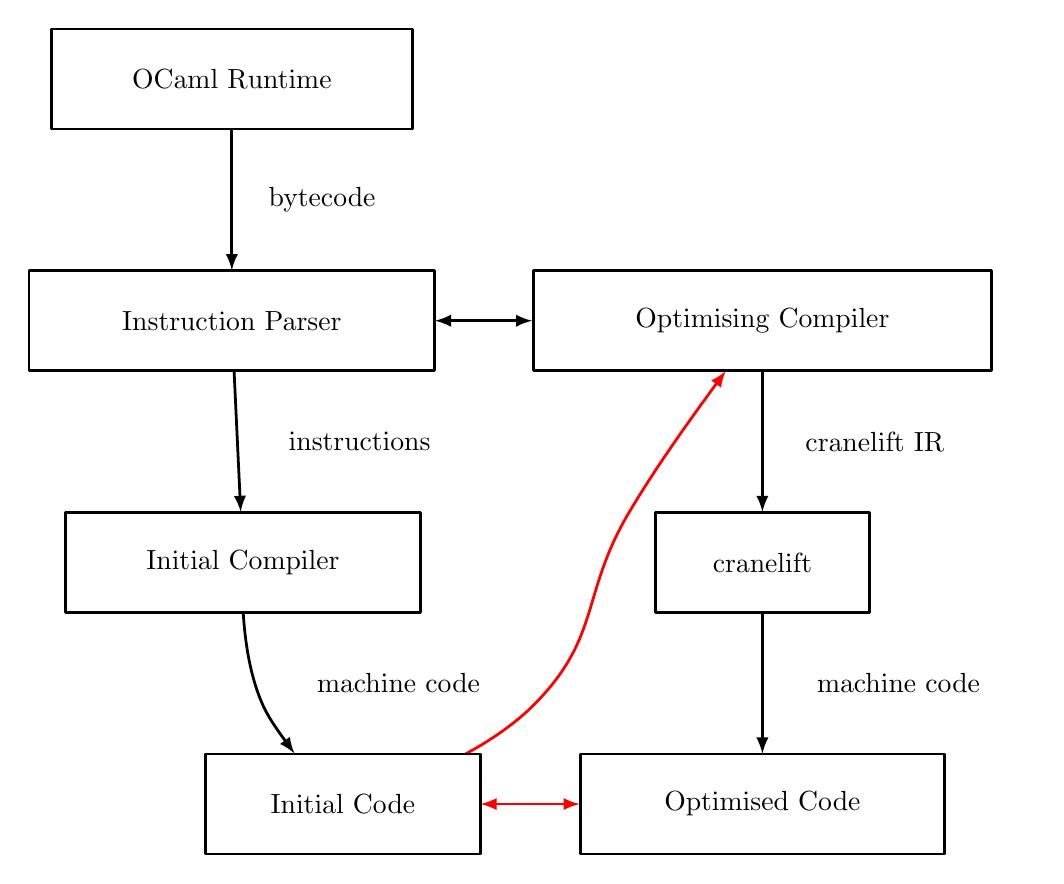
\begin{tikzpicture}[>=latex,line join=bevel,]
  \pgfsetlinewidth{1bp}
%%
\begin{scope}
  \pgfsetstrokecolor{black}
  \definecolor{strokecol}{rgb}{1.0,1.0,1.0};
  \pgfsetstrokecolor{strokecol}
  \definecolor{fillcol}{rgb}{1.0,1.0,1.0};
  \pgfsetfillcolor{fillcol}
  \filldraw (0.0bp,0.0bp) -- (0.0bp,297.0bp) -- (362.0bp,297.0bp) -- (362.0bp,0.0bp) -- cycle;
\end{scope}
\begin{scope}
  \pgfsetstrokecolor{black}
  \definecolor{strokecol}{rgb}{1.0,1.0,1.0};
  \pgfsetstrokecolor{strokecol}
  \definecolor{fillcol}{rgb}{1.0,1.0,1.0};
  \pgfsetfillcolor{fillcol}
  \filldraw (0.0bp,0.0bp) -- (0.0bp,297.0bp) -- (362.0bp,297.0bp) -- (362.0bp,0.0bp) -- cycle;
\end{scope}
\begin{scope}
  \pgfsetstrokecolor{black}
  \definecolor{strokecol}{rgb}{1.0,1.0,1.0};
  \pgfsetstrokecolor{strokecol}
  \definecolor{fillcol}{rgb}{1.0,1.0,1.0};
  \pgfsetfillcolor{fillcol}
  \filldraw (0.0bp,0.0bp) -- (0.0bp,297.0bp) -- (362.0bp,297.0bp) -- (362.0bp,0.0bp) -- cycle;
\end{scope}
  \pgfsetcolor{black}
  % Edge: ocaml_runtime -> instruction_parser
  \draw [->] (73.0bp,260.8bp) .. controls (73.0bp,249.16bp) and (73.0bp,233.55bp)  .. (73.0bp,210.18bp);
  \definecolor{strokecol}{rgb}{0.0,0.0,0.0};
  \pgfsetstrokecolor{strokecol}
  \draw (105.5bp,235.5bp) node {bytecode};
  % Edge: instruction_parser -> optimising_compiler
  \draw [<->] (146.12bp,192.0bp) .. controls (161.16bp,192.0bp) and (166.08bp,192.0bp)  .. (181.11bp,192.0bp);
  % Edge: instruction_parser -> initial_compiler
  \draw [->] (73.809bp,173.8bp) .. controls (74.357bp,162.16bp) and (75.092bp,146.55bp)  .. (76.192bp,123.18bp);
  \draw (119.0bp,148.5bp) node {instructions};
  % Edge: optimising_compiler -> cranelift
  \draw [->] (264.0bp,173.8bp) .. controls (264.0bp,162.16bp) and (264.0bp,146.55bp)  .. (264.0bp,123.18bp);
  \draw (304.5bp,148.5bp) node {cranelift IR};
  % Edge: cranelift -> optimised_code
  \draw [->] (264.0bp,86.799bp) .. controls (264.0bp,75.163bp) and (264.0bp,59.548bp)  .. (264.0bp,36.175bp);
  \draw (313.0bp,61.5bp) node {machine code};
  % Edge: initial_compiler -> compiled_code
  \draw [->] (77.103bp,86.699bp) .. controls (77.721bp,76.765bp) and (79.471bp,64.265bp)  .. (84.0bp,54.0bp) .. controls (85.445bp,50.724bp) and (87.289bp,47.51bp)  .. (95.546bp,36.228bp);
  \draw (133.0bp,61.5bp) node {machine code};
  % Edge: compiled_code -> optimising_compiler
  \pgfsetcolor{red}
  \draw [->] (157.08bp,36.003bp) .. controls (166.06bp,40.865bp) and (174.92bp,46.835bp)  .. (182.0bp,54.0bp) .. controls (206.03bp,78.314bp) and (198.53bp,93.611bp)  .. (216.0bp,123.0bp) .. controls (224.7bp,137.63bp) and (235.56bp,153.2bp)  .. (250.79bp,173.89bp);
  % Edge: compiled_code -> optimised_code
  \draw [<->] (162.55bp,18.0bp) .. controls (177.79bp,18.0bp) and (182.99bp,18.0bp)  .. (198.21bp,18.0bp);
  % Node: instruction_parser
\begin{scope}
  \definecolor{strokecol}{rgb}{0.0,0.0,0.0};
  \pgfsetstrokecolor{strokecol}
  \draw (146.0bp,210.0bp) -- (0.0bp,210.0bp) -- (0.0bp,174.0bp) -- (146.0bp,174.0bp) -- cycle;
  \draw (73.0bp,192.0bp) node {Instruction Parser};
\end{scope}
  % Node: optimising_compiler
\begin{scope}
  \definecolor{strokecol}{rgb}{0.0,0.0,0.0};
  \pgfsetstrokecolor{strokecol}
  \draw (346.5bp,210.0bp) -- (181.5bp,210.0bp) -- (181.5bp,174.0bp) -- (346.5bp,174.0bp) -- cycle;
  \draw (264.0bp,192.0bp) node {Optimising Compiler};
\end{scope}
  % Node: cranelift
\begin{scope}
  \definecolor{strokecol}{rgb}{0.0,0.0,0.0};
  \pgfsetstrokecolor{strokecol}
  \draw (302.5bp,123.0bp) -- (225.5bp,123.0bp) -- (225.5bp,87.0bp) -- (302.5bp,87.0bp) -- cycle;
  \draw (264.0bp,105.0bp) node {cranelift};
\end{scope}
  % Node: initial_compiler
\begin{scope}
  \definecolor{strokecol}{rgb}{0.0,0.0,0.0};
  \pgfsetstrokecolor{strokecol}
  \draw (141.0bp,123.0bp) -- (13.0bp,123.0bp) -- (13.0bp,87.0bp) -- (141.0bp,87.0bp) -- cycle;
  \draw (77.0bp,105.0bp) node {Initial Compiler};
\end{scope}
  % Node: compiled_code
\begin{scope}
  \definecolor{strokecol}{rgb}{0.0,0.0,0.0};
  \pgfsetstrokecolor{strokecol}
  \draw (162.5bp,36.0bp) -- (63.5bp,36.0bp) -- (63.5bp,0.0bp) -- (162.5bp,0.0bp) -- cycle;
  \draw (113.0bp,18.0bp) node {Initial Code};
\end{scope}
  % Node: optimised_code
\begin{scope}
  \definecolor{strokecol}{rgb}{0.0,0.0,0.0};
  \pgfsetstrokecolor{strokecol}
  \draw (329.5bp,36.0bp) -- (198.5bp,36.0bp) -- (198.5bp,0.0bp) -- (329.5bp,0.0bp) -- cycle;
  \draw (264.0bp,18.0bp) node {Optimised Code};
\end{scope}
  % Node: ocaml_runtime
\begin{scope}
  \definecolor{strokecol}{rgb}{0.0,0.0,0.0};
  \pgfsetstrokecolor{strokecol}
  \draw (138.0bp,297.0bp) -- (8.0bp,297.0bp) -- (8.0bp,261.0bp) -- (138.0bp,261.0bp) -- cycle;
  \draw (73.0bp,279.0bp) node {OCaml Runtime};
\end{scope}
%
\end{tikzpicture}



I have implemented a Rust static library which is linked in to the OCaml runtime library and
\texttt{ocamlrun} (the interpreter).
\texttt{ocamlrun} hooks into this library when it loads bytecode and when it starts
interpreting it.
If the JIT is enabled (either by setting an environment variable or enabling it by default at
compile time),
when the bytecode load hook is run the \textbf{initial compiler} will execute.

The initial compiler parses the bytecode into a stream of instructions and for each bytecode
instruction
it emits assembly with the same semantics to a buffer. After all code has been emitted (including
headers
and footers with shared routines) relocations are performed and the buffer is marked as executable.

When \texttt{ocamlrun} then calls the hook to start interpretation, the library instead jumps to
this assembly code which then performs the same operations as the interpreter - except that every
instruction has effectively been inlined.

When an OCaml closure is applied\footnote{all non-primitive function calls are translated to
      closure application}
a closure execution count is incremented. Once this count passes a configurable threshold the code
instead
branches in to the \textbf{optimising compiler}.

The optimising compiler operates on the level of a single function. It starts by doing a
depth-first search to discover all the basic blocks in the function. It then iterates over this
again producing Cranelift IR Format (CLIF) which is passed to the machinery of
\textbf{cranelift}. The CLIF code produced abstracts away the use of the stack allowing cranelift
to perform its register allocation. The function's code pointer is updated and any future calls
(including the originally triggering call) will use the optimised implementation.

\section{Major milestones}

The focus throughout all aspects of the project was focusing on working code that could be tested
even if the total wasn't complete. However it is worth noting the major milestones where some
degree of completeness was achieved. These entries are listed in chronological order.

\begin{enumerate}
      \item Execution of Hello World with the JIT
      \item Passing the OCaml test suite and bootstrapping the compiler
      \item Implementing the benchmark suite
      \item (Extension) Developing the advanced disassembler tools
      \item (Extension) Implementing the optimising compiler
\end{enumerate}

\section{Repository overview}

A more complete overview of the repository is given in section \ref{repo}. However, it is worth
drawing attention to which components are solely, partially or not at all my own work:

\dirtree{%
      .1 /.
      .2 benchmarks.
      .3 sandmark\DTcomment{fork of Sandmark with large patches}.
      .3 analysis\DTcomment{Jupyter notebooks analysing benchmark results}.
      .2 docs\DTcomment{{\LaTeX} source of proposal, report and this document}.
      .2 scripts\DTcomment{scripts to run tests and graph basic blocks}.
      .2 src.
      .3 rust.
      .4 ocaml-jit-shared\DTcomment{shared library between the other two crates}.
      .4 ocaml-jit-staticlib\DTcomment{crate linked in to OCaml runtime}.
      .4 ocaml-jit-tools\DTcomment{binary crate with standalone development/testing tools}.
      .3 ocaml\DTcomment{fork of OCaml compiler 4.11.1}.
      .4 runtime\DTcomment{contains most large patches for the JIT}.
      .3 vendor\DTcomment{vendored rust dependencies with small patches}.
      .2 test-programs\DTcomment{OCaml source for the test programs used by the scripts}.
      .2 vendor/no-aslr\DTcomment{A simple wrapper to run a program without ASLR}.
}

\section{Initial compiler}

The initial compiler was developed first before any work on the optimising compiler was done. In
the process of implementing the
initial compiler some modifications had to be made. These modifications will be covered later in
section \ref{dyn-recomp} and this section will mainly cover the initial state

\subsection{Overview}

The basic compiler consists of two larger components - an instruction parser and an assembly
emitter.

Most of the rest of the files are support for these components and deal with the FFI from and into
the existing runtime.

\subsubsection{Mapping of OCaml abstract machine}

The initial compiler operates by converting every bytecode instruction into a stream of assembly
instructions with the same semantics. Abstract machine registers are mapped to x86\_64 registers. A
pointer to the \texttt{Caml\_state} struct containing other global interpreter state is also
stored in a register called \texttt{r\_cs} for access to its fields with small code size. The
mapping used is shown in Table \ref{table:regmap}.

\begin{table}[h]
      \centering
      \begin{tabular}{cc}\toprule
            OCaml register          & x86\_64 register \\
            \midrule                                   \\
            \texttt{r\_env}         & \texttt{r12}     \\
            \texttt{r\_accu}        & \texttt{r13}     \\
            \texttt{r\_extra\_args} & \texttt{r14}     \\
            \texttt{r\_sp}          & \texttt{r15}     \\
            \texttt{r\_cs}          & \texttt{rbx}     \\
            \bottomrule
      \end{tabular}

      \caption{Mapping of OCaml to x86\_64 registers}
      \label{table:regmap}
\end{table}

Note that all x86\_64 registers mapped are callee-saved in the System V C calling convention. This
means that no work needs to be done spilling and restoring them from the C stack to call C/Rust
primitives (either as part of \texttt{CCall*} instructions or supporting primitives written for the
JIT).

\subsubsection{Mapping of the PC}

Bytecode pointers are mapped to native code pointers and the interpreter's PC is replaced with the
system's instruction pointer. This change is responsible for nearly all of the performance
improvements of the JITed code. The benefits are

\begin{itemize}
      \item Memory accesses are reduced - rather than loading operands and opcodes, they are baked
            in to the machine code
      \item The CPU can predict execution and fill its pipeline further than it can with the use of
            native code pointers
      \item Branch prediction in hot paths become more effective as each branch can be predicted
            differently
      \item Likewise, the CPU can schedule out-of-order execution more effectively across different
            instructions
\end{itemize}

However, this approach does lead to more contention on the instruction cache - rather than only
containing a single copy of the implementation of each instruction there are many.

\codesubsection{Hooks from OCaml}{src/rust/ocaml-jit-staticlib/src/c\_entrypoints.rs}

The existing OCaml runtime was modified to hook into the JIT at three points:

\begin{enumerate}
      \item After a bytecode section is loaded
      \item Before a bytecode section is released
      \item When the interpreter is called
\end{enumerate}

In most programs there are only 1\footnote{or 2 if callbacks from C to OCaml are used} sections
loaded. However, the interpreter is used in other places such as the toplevel REPL which motivates
the more general multiple section support.

Compilation happens after the first hook and an entry is written to a global table containing the
pointer to the buffer. The compiled code takes the form of a single large C function taking no
arguments.

When a section is released this entry is dropped which frees the memory.

The interpreter call hook then calls the JIT-compiled function representing that section.

\subsection{Instruction parsing}

The first stage in the pipeline is to parse the bytes into a stream of elements of the
\texttt{Instruction} type.

\codesubsubsection{The \texttt{Instruction}
      type}{src/rust/ocaml-jit-shared/src/instructions/types.rs}
\label{instruction-type}

OCaml has 149 opcodes, each of which can take different number of operands. Arguments and operands
are all stored as \texttt{i32} values. Rust has good support for algabreic sum types called enums
(which are much more general than the enums in a language like C).

Some of these opcodes are code-size optimisations which represent the composition of multiple
consecutive instructions or have a specific hard-coded operand value. For example,
\texttt{PUSHACC2} represents \texttt{PUSH} then \texttt{ACC2}. \texttt{ACC2} itself is a
specialisation of the more general \texttt{ACC(n)} instruction. These peephole-optimisation
enabling instructions make less sense for the purposes of our interpreter so only the simplest
instructions are considered.

Likewise, there are instructions like integer comparisons and conditional branches that have many
different variations changing only on the exact conditional used.

The instruction type is polymorphic over the type of the label to allow for different label
representations.

\codesubsubsection{Parser}{src/rust/ocaml-jit-shared/src/instruction/parse.rs}

The parser is implemented using Rust iterators; the parser takes an iterator of \texttt{i32}s and
produces an iterator producing values of type \texttt{Result<Instruction,
      ParseError>}\footnote{standard rust error handling type defined as \texttt{enum Result<T,E>
            \{Ok(T), Err(E)\}} like OCaml's \texttt{type ('a, 'b) result = Ok of 'a | Err of 'b}}.

This use of iterators makes the instruction parser consistently performant for large bytecodes -
consumers of the instruction stream take each instruction as they need it.

Labels are stored in the OCaml bytecode as indirect offsets relative to the current PC. To simplify
later uses, these are converted to absolute offsets relative to the start of the section.

As mentioned, single OCaml instructions may parse to more than one \texttt{Instruction}s. To
support this, the type contains a pseudo-instruction called \texttt{LabelDef} which is emitted at
the start of every OCaml instruction. This also allows building a map from OCaml bytecode
absolute offsets to parsed \texttt{Instruction}s.

\codesubsection{Code generation}{src/rust/ocaml-jit-staticlib/src/compiler/emit\_code.rs}

The code generation is the largest aspect of the compiler. It makes use of the \texttt{dynasm-rs}
library. This library manages emitting machine code and relocation information, relocating and
using \texttt{memmap} to mark the code as executable.

The compiler is triggered on the first time a `section' is loaded - for normal programs this is at
startup and for programs using the OCaml toplevel REPL this is after every statement is typed.

The compiler first emits a standard function header entrypoint which saves callee-saved registers
used by the compiler and aligns the C stack. A longjmp handler is set up for exceptions and then
for each bytecode instruction assembly with the same semantics is emitted.

During this process \texttt{dynasm-rs} dynamic labels are used to set up relocations: these
labels are defined before every bytecode instruction and can be referenced by any other
instruction. DynASM translates these at runtime into pc-relative jumps.

After all instructions are done, some shared code used by the instructions is emitted.
\texttt{dynasm-rs} then performs relocations and uses \texttt{mmap} to mark the region of code as
executable.

The overall signature of the assembly produced by this process is a single function taking no
arguments and returning an OCaml value. OCaml closure applications (function calls) do not produce
a stack frame on the C stack - the existing machinery using the OCaml stack is used instead.

\subsubsection{Simple example}

The main code of the compiler itself is contained in a 2000 line file
(\texttt{src/rust/ocaml-jit-staticlib/src/compiler/emit\_code.rs}). Most of this is taken up by a
Rust large pattern match for each of the bytecode instructions. As a very simple example of what
the code looks like consider the implemenation of the \texttt{Add} instruction. It adds the value
at the top of the OCaml stack to the accumulator and stores the result in the accumulator. Note
that the OCaml integer format means a decrement is required. In the original assembler it is
implemented as so:

\inputminted{c}{snippets/add.c}

In the compiler the case becomes:

\inputminted{rust}{snippets/add.rs}

This has exactly the same semantics. Note \texttt{r\_accu} and \texttt{r\_sp}
are aliases for \texttt{r13} and \texttt{r15}.

At compile time, the macro component of \texttt{dynasm-rs} translates it to:

\inputminted{rust}{snippets/add_comp.rs}

Most assembly work is done at compile time - the byte string above contains the machine code for
those instructions. This helps a lot with the performance of the compiler.

\subsubsection{Branches}

For example of the label and relocation support, consider the \texttt{BranchCmp(Comp, i32, L)}
instruction. It
compares the current value of the accumulator to the \texttt{i32} constant using the condition (of
type \texttt{enum Comp {Lt, Gt, ... }}). If the condition is true it branches to the label,
otherwise it passes to the next instruction.

This is implemented as so:

\inputminted{rust}{snippets/branchcmp.rs}

The macros translate it to:

\inputminted{rust}{snippets/branchcmp_comp.rs}

This shows the assembler work still needing to be done at compile time - relocations.

\subsubsection{Other cases}

Most other cases follow these patterns. Some more involved instructions will call into C primitives
I wrote instead (passing and then restoring the registers from the stack).

However, the basic structure of snippets of combined assembly and rust in a large pattern match
statement remains for all cases.

\subsection{Futher details}

Although the basic structure as described holds, some details are omitted but appear in
\texttt{emit\_code.rs}.

\begin{itemize}
      \item There is extensive optional support to support tracing instructions and events
            (described
            in section \ref{tracing})
      \item Callbacks from C to OCaml code require special handling
      \item The compiler returns a pointer to the first instruction to support OCaml's
            metaprogramming \texttt{ocaml\_reify\_bytecode} program used in the implementation of
            things like the
            toplevel \texttt{ocaml} program.
      \item Function application is a fairly involved process and there are checks to resize the
            stack and check for signals as well as the fundamental complexity of the push-enter
            model.
      \item Registers need to be saved and restored at safepoints to allow the garbage collector to
            use them
      \item Certain operations are involved enough that instead of inline the definition in
            hand-written assembly, I push the registers to the C stack and call a C primitive to
            implement the
            operation (taking the registers as a struct)
      \item The compiler stores a persistent data structure of the sections to allow mapping
            bytecode addresses to machine code addresses and allow for cleanup after a section is
            freed.
\end{itemize}

\section{Extension}

Once the initial compiler was complete there was time to dedicate to a significant extension.
Although the initial compiler was performant, it lacked any optimisations between multiple
instructions.

The proposal lists a few ideas of extensions but does not commit to any one of them. Of these, the
decision made would be to focus on combining two concepts:

\begin{itemize}
      \item Dynamic recompilation of hot functions with more optimised forms
      \item Replacing the use of the stack with registers
\end{itemize}

The details of the first extension are explained later in section \ref{dyn-recomp} and the second
extension forms the basis of the optimised compiler described in section \ref{opt-comp}.

\section{Dynamic recompilation} \label{dyn-recomp}

\subsection{Motivations}

Although the initial compiler is impressive there is nothing that could not inherently be done
ahead-of-time. The main benefit to operating as a JIT is it allows for OCaml toplevel sessions to
be
JIT-compiled.

The structure of the bytecode means it is natural to make the optimised compiler operate at the
granularity of a whole function, rather than a basic block or execution trace.	Counting calls and
only branching to the optimising compiler above a certain threshold is a natural method for
determining hot functions and the method I decided to use.

However, allowing this required some changes to the initial compiler. In order to explain these
changes I will first need to give an overview of how the OCaml interpreter deals with efficient
implementation of multiple arguments in the context of a functional language with partial
application.

\subsection{Existing OCaml calls} \label{exist-ocaml}

All functions in OCaml are implemented as closures - a heap allocated tuple of a code pointer and a
list of data.

Function calls look something like this:

\begin{minted}{c}
check_stacks_and_signals(regs);
struct closure *c = (struct closure *) regs->env;
call_function(regs, f->code_ptr);
\end{minted}

Note the actual call logic is done in hand-written assembly and these structs do not exist anywhere
- this and subsequent examples are just pseudo-code. However, it is easier to understand the logic
at a higher level. \texttt{regs} is a pointer to a struct containing the OCaml registers - in the
actual assembly these are machine registers.

\subsubsection{Partial applications}

OCaml uses curried arguments allowing for the use of partial application:

\begin{minted}{ocaml}
# let add a b = a + b
val add : int -> int -> int = <fun>
# add 2 3
- : int = 5
# let add3 = add 3
val add3: int -> int = <fun>
# add3 5
- : int = 8
\end{minted}

In order to avoid making too many intermediate closures, OCaml has special support for this
extensively used pattern. All arguments are passed in order on the stack and the
\texttt{extra\_args}
register is used to mark how many arguments were used.

The number of arguments passed minus 1 is stored in the \texttt{extra\_args} register. The compiler
will insert a \texttt{GRAB(req\_extra\_args)} instruction at the start of any functions which take
more than one argument.

This instruction will return immediately from the function if \texttt{extra\_args} <
\texttt{passed\_extra\_args}. The return value will be a closure itself - this represents partial
application of curried functions. The data of this closure will be the arguments that were passed.
The code pointer of this returned closure points to a \texttt{RESTART} opcode immediately
preceeding the grab, which moves the passed arguments off of the closure's data section onto the
stack, sliding them on top of any additional arguments passed.

Otherwise, it will subtract \texttt{required\_extra\_args} from the \texttt{extra\_args} register
and continue executing.

This model is categorised as a push-enter model because it is the responsibility of the callee to
deal with arity mismatches.

% \subsubsection{Returns}

% Another way we could have written the above example is explicitly curried:

% \begin{minted}{ocaml}
% # let add' a =
% printf "Making an adder with %d\n";
% fun b -> a + b
% val make_adder : int -> int -> int = <fun>
% # let add3 = add' 3
% Making an adder with 3
% val add3 : int -> int = <fun>
% # add3 5
% - : int = 8
% # add' 2 4
% Making an adder with 2
% - : int = 6
% \end{minted}

% Although this looks similar, OCaml can no longer use the partial application support. Rather than
% compiling this to one function taking two arguments, it is forced by the print statement to compile
% it to a function taking one argument and returning a function. These are semantically the same but
% differ in implementation.

% The key opcode is the \texttt{Return} instruction which like \texttt{Grab} behaves differently based
% on the value of \texttt{extra\_args}.

% If \texttt{make\_adder} is called with one argument (\texttt{extra\_args} = 0), it will return the
% closure. However if \texttt{make\_adder} is called with two arguments, \texttt{extra\_args} will be 1.

% \texttt{Return} will check if \texttt{extra\_args} $> 0$ and if so will try to call the return value
% with the additional arguments.

\subsection{Function table}

In order to support dynamic recompilation it is necessary to store the call count somewhere. A
naive method would be to store this in the closure as an extra data item, but this cannot support
optimising cases where the same code is used with different closure environments.

Instead, I modified the code pointer to point to a structure in memory. This structure is shared
between all closures using the same code. For now imagine it contains only one field: the code
pointer.

Calls became:

\begin{minted}{c}
check_stacks_and_signals(regs);
struct closure *c = (struct closure *) regs->env;
struct function_metadata *f = c->code_ptr;
call_function(regs, f->code);
\end{minted}

\subsection{Moving the responsibility to the caller - eval/apply model}

I do not wish for optimised functions to do any of the work described in section \ref{exist-ocaml}.
As is described later, most of the speed increases of the optimised compiler comes from completely
eliminating use of the OCaml stack and the call method above makes heavy use of it.

Instead I shift the work to logically be done by the caller. The way this is done is by adding a
field storing \texttt{required\_extra\_args} to the function table and transorming the function
code call to look something like this:

\begin{minted}{c}
check_stacks_and_signals(regs);
struct closure *c = (struct closure *) regs->env;
struct function_metadata *f = c->code_ptr;
if (regs->extra_args < f->required_extra_args) {
      // return partial application doing work of GRAB
} else {
      regs->extra_args -= f->required_extra_args;
      call_function(regs, f->code);
}
\end{minted}

I then modified the assembly translation of \texttt{GRAB} to be a no-op. The exact same work is
performed but now it is the responsibility of the caller.

\subsection{Call counts and dynamic recompilation}

I added two new fields to the function table struct: a reference to the original bytecode location
of the function and a count/status variable.

The count/status is initialised to 0. Calls become:

\begin{minted}{c}
check_stacks_and_signals(regs);
struct closure *c = (struct closure *) regs->env;
struct function_metadata *f = c->code_ptr;
if (regs->extra_args < f->required_extra_args) {
      // return partial application doing work of GRAB
} else { 
      regs->extra_args -= f->required_extra_args;
      if (f->count_status == -1) {
            // Call the optimised function
            call_opt(regs, f->code);
      } else if (f->count_status == THRESHOLD_CALLS) {
            // Run the optimising compiler then call the optimised function
            f->code = optimising_compiler(f->original_bytecode_location);
            f->count_status = -1;
            call_opt(regs, f->code);
      } else {
            // Increment count and call the unoptimised function 
            f->count_status++;
            call_function(regs, f->code);
      }
}
\end{minted}

\subsection{Actual implementation}

Even though most of the above snippets are pseudo-code the function metadata struct as listed with
its four fields (code pointer, original bytecode location, required extra args, count/status)
actually exists. The initial compiler was first modified to generate, store and use it.

In order to generate this, I added another pass to the initial compiler which discovers the
bytecode locations of all closures. This is done by iterating through all functions. When a
\texttt{Closure(bytecode\_location, num\_vars)} bytecode operation is found (which creates a
closure) the code pointer is inspected. By inspecting the first instruction found at the bytecode
location, it is possible to find the value of the \texttt{required\_extra\_args} field.

After all the code is emitted, the function table is emitted. \texttt{dynasm-rs}'s relocations are
used to load the initial code pointers into the function table and link to the struct in the
closure table when compiling \texttt{Closure(...)} operations.

Due to the change from single to double level of pointer indirection for function calls these
changes added some overhead. However they were

\section{Optimising compiler} \label{opt-comp}

\subsection{Motivation and design}

We have from the work in the previous section a way to determine hot closures and dynamically call
into an optimising compiler. This section describes the implementation of this optimising compiler
and how calls are done.

The time left meant building a complete x86\_64 compiler backend (with register allocation,
instruction selection, etc.) from scratch was infeasible. The usual toolkit used to avoid
replicating this work is LLVM \cite{llvm}. Although is more typically known for its use in
ahead-of-time compilation, there is support for use in JITs.

\subsubsection{Problems with LLVM}

I initially decided to go with LLVM but as the implementation started I ran into some limitations.

\begin{itemize}
      \item LLVM is very large and bloated - compiling it with multiple jobs caused my machine to
            run out of memory and linking it in massively bloated the binary size of
            \texttt{ocamlrun}
      \item The safepoint GC support while somewhat mature is messy and would require writing
            patching the C++ source of LLVM to add new options as well as diving very deep into
            internal data
            structures
      \item Although there are some very good Rust bindings, not all features of the C++ api are
            exposed. This is especially true with the garbage collector support.
      \item LLVM has about 2 different JIT interfaces (\texttt{MCJit}, \texttt{orc},
            \texttt{orcv2}),
            all of which had different limitations when used in a project such as mine and only
            \texttt{MCJit} had good Rust bindings
      \item LLVM is somewhat heavyweight and compilation is slow which means there is a large risk
            of slower overall performance even if only compiling hot functions.
\end{itemize}

\subsubsection{Cranelift}

After struggling with these issues I discovered the \texttt{cranelift} project. Like LLVM it is a
retargetable code generator with an IR. However, it has a number of different design decisions
which made it much better suited for my planned uses:

\begin{itemize}
      \item It is written in Rust which means the API is fairly idiomatic when using it in Rust
      \item It is designed primarily for JITs and focuses heavily on compilation performance
      \item The project is actively developed and I could communicate with the developers when I
            had
            questions who were very responsive.
      \item Although the support for garbage collection is not as extensible, with the help of the
            developers I was able to come up with a model that is a good fit for the OCaml garbage
            collector's
            requirements.
      \item When I encountered any bugs or missing features I could easily submit and get merged
            patches to the project which uses a familiar Github workflow rathter than the LLVM
            project's legacy
            systems.
\end{itemize}

There were still some missing features in Cranelift which are described later but for the most
part it was a good fit for my needs and was in a large part responsible for my being able to
complete this ambitious extension.

\subsection{Overview}

At a high level the optimised compiler is a function taking two inputs and returning two outputs.
The inputs are a slice to the code of a section of a bytecode, and the offset within that slice
containing the
first instruction in the function to be optimised.

The first output is a pointer to a compiled function that can be called to execute the code
represented by that function. The second output is a vector of stack map entries which are used
to support finding GC roots (explained in \ref{optgc}). The first output becomes the new code
pointer
in the function metadata table.

The compiler consists of three major components.

\begin{enumerate}
      \item Basic block conversion and stack start analysis (section \ref{opt-bb})
      \item IR generation from the basic blocks using the analysis (section \ref{opt-irgen})
      \item Compilation of IR to x86\_64 assembly (done by Cranelift)
\end{enumerate}

As described later in section \ref{dyn-recomp}, this compiler is triggered once a function is
called enough times to become `hot'. After the function is compiled the optimised implementation
will always be used.

\subsection{Changes}

The largest change from the initial compiler to the optimised compiler is the removal of
use of the OCaml stack and accumulator registers. This is done by replacing these uses of the OCaml
stack with machine registers and the C stack.

Arguments are passed to a function according to the System V C calling convention - the first
argument is always the closure environment, \texttt{env}, and the remaining arguments are passed
in registers. Direct calls from optimised functions to optimised functions can avoid the use of
the OCaml stack entirely. Other cases need more work (described in section \ref{dyn-recomp}).

The method used to remove the use of the stack is to convert the OCaml bytecode into an SSA form
by keeping track of the contents of a virtual stack and accumulator as the closure is translated.
As an example consider the simple OCaml function:

\mint{ocaml}|let add a b = a + b|

This compiles to the sequence of bytecode instructions:

\begin{verbatim}
Grab(1)          # Ensure 2 arguments passed
Acc(1)           # Load 2nd element from top of stack to acc
Push             # Push acc
Acc(1)           # Load new 2nd element from top of stack to acc
ArithInt(Add)    # Add top of stack to the acc and pop it
Return(2)        # Pop 2 items, then return acc
\end{verbatim}

Instead of translating all of these inefficient stack manipulations as the initial compiler does,
the optimised compiler keeps track of the stack as it compiles. For an example of this, see table
\ref{table:stacktrans}. Ignore the \texttt{Grab(1)} for
now as it is handled in a different way.

\begin{table}[h]
      \centering
      \begin{tabular}{ccc}\toprule
            Initial state                   & Operation              & Final state
            \\
            \midrule
            \\
            \texttt{acc=?, stack=[b, a]}    & \texttt{Acc(1)}        & \texttt{acc=a, stack=[b, a]}
            \\
            \texttt{acc=a, stack=[b, a]}    & \texttt{Push}          & \texttt{acc=a, stack=[a, b,
                              a]}
            \\
            \texttt{acc=a, stack=[a, b, a]} & \texttt{Acc(1)}        & \texttt{acc=b, stack=[a, b,
                              a]}
            \\
            \texttt{acc=b, stack=[a, b, a]} & \texttt{ArithInt(Add)} & \texttt{acc=a+b, stack=[b,
                              a]}
            \\
            \texttt{acc=a+b, stack=[b, a]}  & \texttt{Return(2)}     & \texttt{acc=a+b, stack=[]}
            \\
            \bottomrule
      \end{tabular}

      \caption{Translation of add}
      \label{table:stacktrans}
\end{table}

This method is effective when considering a single basic block at a time. However, in the presence
of branching, joining and looping basic blocks more work is needed. Luckily the output of the OCaml
compiler has the invariant that the stack size relative to the function's stack frame is constant
at the start of each basic block, \emph{no matter the path taken to reach it}. This happens to be
the key to allow efficient SSA conversion, completely removing any explicit notion of a stack and
accumulator from the generated Cranelift IR.

\codesubsection{Conversion to basic blocks}{src/rust/ocaml-jit-shared/src/basic\_blocks/}
\label{opt-bb}

The typical data structure used in optimising compilers is the basic block. \emph{Make sure I've
      defined this somewhere in preparation}.

However, the only information we have from the bytecode is a sequence of instructions with jumps.
In order to move away from a heavy connection with the instructions the first step is to decompile
to basic blocks.

\codesubsubsection{Types}{basic\_blocks/types.rs}

A \textbf{\texttt{BasicClosure}} consists of a vector of \textbf{\texttt{BasicBlock}} along with
some other data. A basic block has a vector of \textbf{\texttt{BasicBlockInstruction}} and a single
\textbf{\texttt{BasicBlockExit}}.

Some \texttt{Instruction}s (see section \ref{instruction-type}) map to a
\texttt{BasicBlockInstruction} and others map to a \texttt{BasicBlockExit}. For example,
\texttt{Instruction::Push} becomes \texttt{BasicBlockInstruction::Push} but
\texttt{Instruction::BranchIf(label)} becomes \texttt{BasicBlockExit::BranchIf { then\_block,
else\_block }}.

This enforces at the type level the basic invariant of basic blocks - one entry, one exit.

\subsubsection{Stack starts}

In addition to performing the conversion to basic blocks, the algorithm also keeps track of a
concept I call the \textbf{stack start} of a basic block. Although, like all other aspects of the
OCaml interpreter, it is not documented anywhere, inspecting the bytecode compiler's source and
testing against all real programs finds an important invariant:

For all paths leading from the entry block of a function to an instruction, the absolute stack size
relative to the start of the function's stack frame is the same.

During the conversion to basic blocks this invariant is validated and the size of the stack before
the first instruction of a block (the stack start) executes. This is the \textbf{stack start} of
the block.

\codesubsubsection{Algorithm}{basic\_blocks/conversion.rs}

The algorithm consists of two runs of DFS. The first finds all bytecode offsets which form the
start of blocks. The second visits all these blocks working out stack sizes.

In order to describe this algorithm without too many confusing details I will create a formalism
just complicated enough to include all the complexity.

The first DFS pass is only necessary to deal with loop back edges. For simplicity let's assume this
doesn't happen.

Let \(I\) be the set of all instructions. The program \(P\) is a list of instructions and can be
indexed. For simplicity, assume indices are consecutive\footnote{they're not but it's fairly simple
      to handle}.

Each instruction has four properties:

\begin{itemize}
      \item \(\delta(i)\) is the change to the stack pointer after executing the instruction. For
            example \texttt{Push} which pushes the acc to the stack has \(\delta(\texttt{Push}) =
            +1\)
      \item \(\dfsexit(i)\) returns \textbf{true} iff the instruction causes the block to end
            (jumps, returns)
      \item \(\dfsfallthrough(i)\) returns \textbf{true} iff \(\dfsexit(i)\) and it can end up
            jumping to the following instruction. \texttt{BranchIf(branch\_loc)} is fallthrough but
            \texttt{Branch(branch\_loc)} is not.
      \item \(\dfslabels(i)\) returns a set of all labels the instruction could end up jumping to
            (not
            including fallthrough). For example \(\dfslabels(\texttt{BranchIf(branch\_loc)}) =
            \{\text{branch\_loc}\}\). It is only relevant if \(\dfsexit(i)\)
\end{itemize}

Under this model, the algorithm to find all the blocks and their starts is shown in algorithm
\ref{alg-dfs}. The actual algorithm is more complicated and calculates more things but not
conceptually any different.

\begin{algorithm}
      \caption{DFS to find basic blocks and their starts}\label{alg-dfs}
      \begin{algorithmic}[1]
            \Function{FindBlocks}{$P, arity$}
            \State $seen \gets \emptyset$
            \State $starts \gets \{\}$
            \Function{VisitBlock}{$initial\_index, initial\_stack\_size$}
            \If{$initial\_index \in seen$}
            \Assert{$starts[initial\_index] = initial\_stack\_size$}
            \State \textbf{return}
            \EndIf
            \State $starts[initial\_index] \gets initial\_stack\_size$
            \State $i \gets initial\_index$
            \State $s \gets initial\_stack\_size$
            \Repeat
            \State $x \gets P[i]$
            \State $s \gets s + \delta(x)$
            \If{$\dfsexit(x)$}
            \For{$j \in \dfslabels(i)$}
            \State \Call{VisitBlock}{j, s}
            \EndFor
            \If{$\dfsfallthrough(x)$}
            \State \Call{VisitBlock}{i + 1, s}
            \EndIf
            \State \textbf{return}
            \EndIf
            \State $i \gets i + 1$
            \Until{forever}
            \EndFunction
            \State \Call{VisitBlock}{0, arity}
            \State \textbf{return} $starts$
            \EndFunction
      \end{algorithmic}
\end{algorithm}

\subsubsection{Additional operations performed during the search} \label{addop}

The algorithm as presented in algorithm \ref{alg-dfs} shows only the basic logic of the search and
storing of the stack starts for each block. The actual search also performs more work:

\begin{itemize}
      \item When a block is visited a vector is created to hold the parsed instructions
      \item Blocks are numbered in reverse post-order (the natural order for basic blocks where
            with the exception of loop back edges, blocks are visited in a way consistent with
            execution order).
      \item Every time an instruction is visit any labels referencing other blocks are replaced
            with the block ids and a copy is added to the vector.
      \item At exit, all of the block metadata is stored in a \texttt{BasicBlock} struct and placed
            in a table of blocks referenced by the block number.
      \item The maximum stack size at any point in the function is computed. It is used later in
            the IR generation phase.
\end{itemize}

\subsubsection{Example}

\subsection{Calling conventions}

In the initial interpreter, all calling is done using the OCaml interpreter's existing model. This
passes all arguments on the OCaml stack and has the caller deal with partial application and tail
calls.

We would like to avoid the stack in hot paths, so instead use an eval-apply model. Arguments are
passed according to the System V calling convention and a function is only called with all the
arguments it expects.

\textbf{TODO: flesh this out with some actual example prototypes}

\subsection{IR generation} \label{opt-irgen}

\textbf{TODO: integrate the examples better}

\subsubsection{Example: Add}

Consider the add function:

\mint{ocaml}|let add a b = a + b|

\begin{verbatim}
Arity: 2
Max stack size: 3

# Block 0 (stack_start = 2)
Acc(1)
Push
Acc(1)
ArithInt(Add)
Exit: Return(2)
\end{verbatim}

\subsubsection{Clamp}

\begin{minted}{ocaml}
(% clamp : int -> int -> int %)
let clamp h l (x : int) =
  if h < x then
    h
  else if l > x then
    l
  else
    x
\end{minted}

\begin{verbatim}
Arity: 3
Max stack size: 4

# Block 0 (stack_start = 3)
Acc(2)
Push
Acc(1)
IntCmp(Lt)
Exit: BranchIf { then_block: 1, else_block: 2 }

# Block 1 (stack_start = 3)
Acc(0)
Exit: Return(3)

# Block 2 (stack_start = 3)
Acc(2)
Push
Acc(2)
IntCmp(Gt)
Exit: BranchIf { then_block: 3, else_block: 4 }

# Block 3 (stack_start = 3)
Acc(1)
Exit: Return(3)

# Block 4 (stack_start = 3)
Acc(2)
Exit: Return(3)
\end{verbatim}


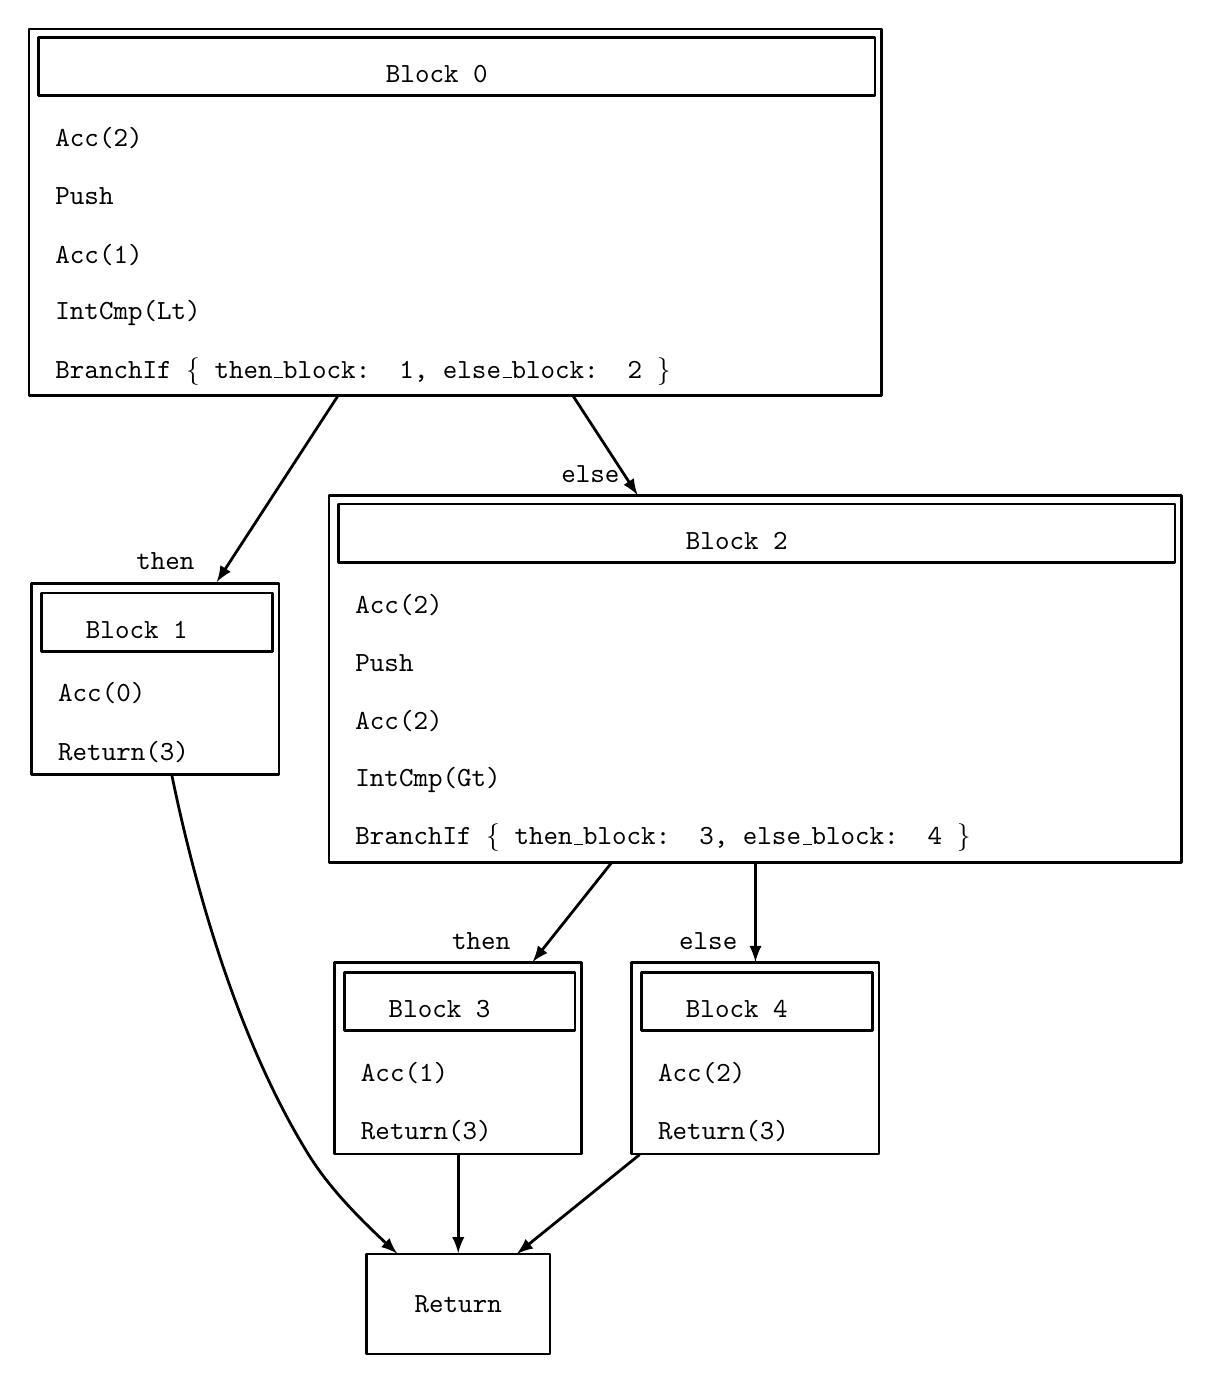
\begin{tikzpicture}[>=latex,line join=bevel,]
  \pgfsetlinewidth{1bp}
\ttfamily%
\pgfsetcolor{black}
  % Edge: n0 -> n1
  \draw [->] (111.13bp,344.87bp) .. controls (98.328bp,325.2bp) and (84.615bp,304.12bp)  .. (67.561bp,277.91bp);
  \definecolor{strokecol}{rgb}{0.0,0.0,0.0};
  \pgfsetstrokecolor{strokecol}
  \draw (49.061bp,285.41bp) node { then};
  % Edge: n0 -> n2
  \draw [->] (195.87bp,344.87bp) .. controls (201.65bp,335.99bp) and (207.61bp,326.82bp)  .. (219.07bp,309.22bp);
  \draw (202.07bp,316.72bp) node { else};
  % Edge: n1 -> return
  \draw [->] (51.405bp,208.35bp) .. controls (58.789bp,172.52bp) and (73.825bp,115.14bp)  .. (100.5bp,72.0bp) .. controls (107.02bp,61.458bp) and (116.07bp,51.486bp)  .. (132.53bp,36.158bp);
  % Edge: n2 -> n3
  \draw [->] (209.57bp,176.72bp) .. controls (202.07bp,167.29bp) and (194.52bp,157.81bp)  .. (181.28bp,141.16bp);
  \draw (162.78bp,148.66bp) node { then};
  % Edge: n2 -> n4
  \draw [->] (261.5bp,176.72bp) .. controls (261.5bp,168.06bp) and (261.5bp,159.36bp)  .. (261.5bp,141.16bp);
  \draw (244.5bp,148.66bp) node { else};
  % Edge: n3 -> return
  \draw [->] (154.5bp,71.809bp) .. controls (154.5bp,63.365bp) and (154.5bp,54.41bp)  .. (154.5bp,36.297bp);
  % Edge: n4 -> return
  \draw [->] (219.82bp,71.809bp) .. controls (207.64bp,61.961bp) and (194.6bp,51.416bp)  .. (175.6bp,36.059bp);
  % Node: n0
\begin{scope}
  \definecolor{strokecol}{rgb}{0.0,0.0,0.0};
  \pgfsetstrokecolor{strokecol}
  \draw (3.5bp,453.0bp) -- (3.5bp,474.0bp) -- (304.5bp,474.0bp) -- (304.5bp,453.0bp) -- cycle;
  \draw (124.5bp,460.8bp) node[right] {Block 0};
  \draw (5.5bp,437.8bp) node[right] {Acc(2)  };
  \draw (5.5bp,416.8bp) node[right] {Push  };
  \draw (5.5bp,395.8bp) node[right] {Acc(1)  };
  \draw (5.5bp,374.8bp) node[right] {IntCmp(Lt)  };
  \draw (5.5bp,353.8bp) node[right] {BranchIf \{ then\_block: 1, else\_block: 2 \}  };
  \draw (0.0bp,345.0bp) -- (0.0bp,477.0bp) -- (307.0bp,477.0bp) -- (307.0bp,345.0bp) -- cycle;
\end{scope}
  % Node: n1
\begin{scope}
  \definecolor{strokecol}{rgb}{0.0,0.0,0.0};
  \pgfsetstrokecolor{strokecol}
  \draw (4.5bp,253.0bp) -- (4.5bp,274.0bp) -- (87.5bp,274.0bp) -- (87.5bp,253.0bp) -- cycle;
  \draw (16.5bp,260.8bp) node[right] {Block 1};
  \draw (6.5bp,237.8bp) node[right] {Acc(0)  };
  \draw (6.5bp,216.8bp) node[right] {Return(3)  };
  \draw (1.0bp,208.5bp) -- (1.0bp,277.5bp) -- (90.0bp,277.5bp) -- (90.0bp,208.5bp) -- cycle;
\end{scope}
  % Node: n2
\begin{scope}
  \definecolor{strokecol}{rgb}{0.0,0.0,0.0};
  \pgfsetstrokecolor{strokecol}
  \draw (111.5bp,285.0bp) -- (111.5bp,306.0bp) -- (412.5bp,306.0bp) -- (412.5bp,285.0bp) -- cycle;
  \draw (232.5bp,292.8bp) node[right] {Block 2};
  \draw (113.5bp,269.8bp) node[right] {Acc(2)  };
  \draw (113.5bp,248.8bp) node[right] {Push  };
  \draw (113.5bp,227.8bp) node[right] {Acc(2)  };
  \draw (113.5bp,206.8bp) node[right] {IntCmp(Gt)  };
  \draw (113.5bp,185.8bp) node[right] {BranchIf \{ then\_block: 3, else\_block: 4 \}  };
  \draw (108.0bp,177.0bp) -- (108.0bp,309.0bp) -- (415.0bp,309.0bp) -- (415.0bp,177.0bp) -- cycle;
\end{scope}
  % Node: return
\begin{scope}
  \definecolor{strokecol}{rgb}{0.0,0.0,0.0};
  \pgfsetstrokecolor{strokecol}
  \draw (187.5bp,36.0bp) -- (121.5bp,36.0bp) -- (121.5bp,0.0bp) -- (187.5bp,0.0bp) -- cycle;
  \draw (154.5bp,18.0bp) node {Return};
\end{scope}
  % Node: n3
\begin{scope}
  \definecolor{strokecol}{rgb}{0.0,0.0,0.0};
  \pgfsetstrokecolor{strokecol}
  \draw (113.5bp,116.5bp) -- (113.5bp,137.5bp) -- (196.5bp,137.5bp) -- (196.5bp,116.5bp) -- cycle;
  \draw (125.5bp,124.3bp) node[right] {Block 3};
  \draw (115.5bp,101.3bp) node[right] {Acc(1)  };
  \draw (115.5bp,80.3bp) node[right] {Return(3)  };
  \draw (110.0bp,72.0bp) -- (110.0bp,141.0bp) -- (199.0bp,141.0bp) -- (199.0bp,72.0bp) -- cycle;
\end{scope}
  % Node: n4
\begin{scope}
  \definecolor{strokecol}{rgb}{0.0,0.0,0.0};
  \pgfsetstrokecolor{strokecol}
  \draw (220.5bp,116.5bp) -- (220.5bp,137.5bp) -- (303.5bp,137.5bp) -- (303.5bp,116.5bp) -- cycle;
  \draw (232.5bp,124.3bp) node[right] {Block 4};
  \draw (222.5bp,101.3bp) node[right] {Acc(2)  };
  \draw (222.5bp,80.3bp) node[right] {Return(3)  };
  \draw (217.0bp,72.0bp) -- (217.0bp,141.0bp) -- (306.0bp,141.0bp) -- (306.0bp,72.0bp) -- cycle;
\end{scope}
%
\end{tikzpicture}



\subsubsection{Cranelift IR basics}

Cranelift, much like LLVM, uses an IR with a binary, in-memory and textual representation. The
basic concept is that of typed values where the types are things like \texttt{I64} and
\texttt{F32}. When constructing IR as part of the frontend, cranelift provides some assistance with
translating dynamic mutable variables to SSA values inserting block parameters where needed.

The basic Rust data type of cranelift IR is a \texttt{Value}. It is returned by most IR builder
functions and used as parameters. Cranelift values have a (cranelift) type but this is not
replicated in the Rust type system.

The individual unit of compilation is the function. Each function has a preamble where it can
declare functions it calls and needs to be linked to, or any pointers of global data needed. This
differs from LLVM where the basic unit of compilation is a module, equivalent to a C object file or
Rust crate, and any imports of things needing relocation is done at the module level. This permits
LLVM to do cross-function optimisation. Cranelift is nowhere near as optimising (and as such
significantly faster for use in JITs) and those it does do are local to the function or basic
block.

\subsubsection{Cranelift's assistance - variables}

Legal Cranelift IR is in strict SSA form using block parameters. It is possible for the frontend
code to build this themselves and for certain primitives doing this manually and managing block
parameters is sensible. However, the abstraction of most imperative programming languages (and the
bytecode output of OCaml) is the use of mutable variables. One reasonable method to compile these
is to allocate storage on the C stack for variables upfront and have accesses use this and
historically this is the method used by compilers. However, we wish to make use of the large number
of registers on modern architectures.

LLVM does this using an optimisation pass called \texttt{mem2reg}. As its name implies, it notices
the pattern of allocating variables upfront and translates them to use registers. It inserts phi
nodes (a precursor of block parameters; block parameters did not exist when LLVM was made) where
necessary.

Cranelift takes a more direct approach based on the 20XX paper from \textbf{find that paper}.
Conversion of variables to use SSA values is done inline with the rest of the IR building using the
elegant online algorithm of Name. The high-level summary is values of type \texttt{Variable} can be
created. During IR generation, \texttt{value = self.builder.use\_var(var)} allows for getting the
current value of a variable at this basic block as something of \texttt{Value} type.
\texttt{self.builder.def\_var(var, value)} allows for setting the value of a variable. Both
functions abstract away the work of keeping track of adding block parameters, dealing with liveness
and translating variable values.

\subsubsection{Translating stack use to variables}

I use this functionality to translate all references to the OCaml stack to values. As mentioned in
section \ref{addop} the DFS search to find all basic blocks and compute stack sizes also stores the
maximum stack size at any point in the function. I allocate this number of \texttt{Variable}s to
create a virtual \texttt{stack}. As code is generated the virtual stack size is managed.
Additionally, a \texttt{Variable} is created to manage the current state of the accumulator.

\subsubsection{Examples}

Although it may seem confusing from this description, this approach is actually very elegant in
practice. Let's consider the \texttt{ArithOp(Add)} example again. As a reminder, it adds the top of
the stack to the current accumulator value (where adding actually requires a decrement).

\begin{minted}{rust}
let a = self.get_acc_int();
let b = self.pick_int(0)?;
self.pop(1)?;

// a is OCaml rep of x, b is OCaml rep of y
// a + b = (x * 2 + 1) + (y * 2 + 1) = (x + y) * 2 + 2
// result = a + b - 1 = (x + y) * 2 + 1
let added = self.builder.ins().iadd(a, b);
let result = self.builder.ins().iadd_imm(added, -1);
self.set_acc_int(result);
\end{minted}

This case is remarkably similar to the case in the original interpreter - however rather than
directly performing the operation it is instead making calls which trigger the emission of IR with
the same semantics.

To show this example in complete context consider the add function:

\mint{ocaml}|let add a b = a + b|

\begin{verbatim}
Arity: 2
Max stack size: 3

# Block 0 (stack_start = 2)
Acc(1)
Push
Acc(1)
ArithInt(Add)
Exit: Return(2)
\end{verbatim}

As it is a function taking two arguments, it is compiled to a function taking 3 arguments - the
closure environment (unused for this function) and the two original arguments, \texttt{a} and
\texttt{b}.

It compiles to something like this\footnote{the actual IR is larger as it uses \texttt{R64} types
      and bitcasts for GC as
      described in section \ref{gc-ir} but the principle is the same}:

\begin{verbatim}
function u0:0(i64, i64, i64) -> i64, i64 system_v {

block0(v0: i64, v1: i64, v2: i64):
    v3 = iconst.i64 0
    v4 = iadd v1, v2
    v5 = iconst.i64 -1
    v6 = iadd v4, v5
    jump block1

block1:
    return v6, v3
}
\end{verbatim}

This is a fairly direct translation of the semantics of the function - without any use of the OCaml
stack!

Cranelift compiles the IR to this machine code. Note: in the System V calling convention, the first
three arguments are passed in \texttt{rdi} and \texttt{rsi}, \texttt{rdx} respectively and return
values (up to 2) are in \texttt{rax} and \texttt{rdx} respectively:

\begin{verbatim}
0000000000000000 <arith_add>:
   0:	55           push   rbp                    ; set up rbp chain
   1:	48 89 e5     mov    rbp,rsp                ;  
   4:	48 01 d6     add    rsi,rdx                ; v4 = v1 + v2
   7:	48 83 c6 ff  add    rsi,0xffffffffffffffff ; v6 = v4 + (v5 = -1)
   b:	48 89 f0     mov    rax,rsi                ; 1st retval = v6
   e:	48 31 d2     xor    rdx,rdx                ; 2nd retval = v3 = 0
  11:	48 89 ec     mov    rsp,rbp                ; restore rbp
  14:	5d           pop    rbp                    ;
  15:	c3           ret    
\end{verbatim}

Apart from the missed peephole optimisation at offset 7\footnote{\texttt{dec rsi} would save a
      byte}, the assembly is very directly what we would expect.

\textbf{TODO - put a more complicated example in the appendix}

\subsubsection{Summary}

The combination of cranelift and my virtual stack allows me to write code which is in mostly 1-1
correspondance with the interpreter source while compiling to register-using optimised machine
code. All of this is done while remaing fairly quick (at least compared to its competitors)

\subsection{GC support} \label{gc-support}

A key aspect of the OCaml runtime is its garbage collection support. In the bytecode interpreter no
particular effort is needed for this as every value is stored on the OCaml stack. However, for my
compiled code which does not use the OCaml stack it is necessary to build something more involved.

As some of the steps are a bit fiddly I will start with an overview of how the steps involved fit
together:

\begin{enumerate}
      \item During cranelift IR generation, I store everything that could contain a pointer to a
            GC-managed value (a \textbf{local root}) in a cranelift \textbf{reference type}
            (\texttt{R64}).
      \item Cranelift performs LVA, spilling and restoring of registers to the C stack and emission
            of \textbf{stack maps} at every GC \textbf{safepoint}.
      \item My runtime stores the stack maps in a hash map keyed by the return address at time of
            the safepoint.
      \item During GC, my runtime walks entire the frame pointer (\texttt{rbp}) chain. By looking
            at the return address and using the hash map to discover any stack maps, my runtime
            tells the OCaml GC about the location and value of any local roots which could contain
            pointers.
\end{enumerate}

I am incredibly grateful for the assistance Nick Fitzgerald, Chris Fallin and other Bytecode
Alliance members who helped me in the Zulip chat to make all this work and reviewed my pull
requests. I am reasonably certain that I am the only non-wasmtime user of cranelift's GC support so
far.

\subsubsection{IR generation} \label{gc-ir}

Cranelift has support for precise garbage collection. It was originally created for webassembly
reference types but luckily mapped well to the needs of OCaml. Precise (sometimes called
\emph{exact} or \emph{accurate}) means that the GC is able to determine all roots and only the
roots
when tracing. The opposite is a \emph{conservative} collector which allows for an over-estimate.

In order to use it my IR generation has to mark roots by storing them in values which have the
\texttt{R64} type. The \texttt{R64} type means 64-bit reference and is compiled identically to
\texttt{I64}. However, cranelift support will use this type to differentiate GC-managed pointers
from other values.

For this reason, anything which is an OCaml value and could be a pointer to the heap \textbf{must}
be stored in a \texttt{R64} type at every point the GC could trigger (a \emph{safepoint}).

However, despite being almost equivalent in implementation to \texttt{I64}s not all operations that
can be done using \texttt{I64} values can be done using \texttt{R64} values. This is only really a
problem because of OCaml's mixed integer/pointer data representation. The integer add operation is
not
implemented for \texttt{R64}s but is needed to add two integers stored in OCaml's uniform
representation.

The somewhat hacky solution I came up with is to use the \texttt{raw\_bitcast} operation to
temporarily convert \texttt{R64} values to \texttt{I64}, perform any arithmatic, and then convert
back.

The key invariant I had to hold to make this work was that these casted \texttt{R64}-derived
\texttt{I64} values were only temporary to the implementaiton of the operation that uses them.

\subsubsection{What cranelift does}

\emph{None of this section is my work (except for my pull requests to Cranelift fixing bugs I
      encountered).}

Cranelift's GC support works using the concept of safepoints. A safepoint is a point in the program
where the garbage collector could run. Cranelift treats every function call as a
safepoint\footnote{I planned a way to make this configurable per-function with the cranelift
      developers but decided it would take too long at the late stage of the project}.

At every safepoint (here function call), cranelift will ensure:

\begin{enumerate}
      \item All live \texttt{R64} values have a copy on the stack so the GC could find them
      \item No code or optimisation assumes that the old value of a \texttt{R64} is still valid
            after the safepoint
\end{enumerate}

In order to determine the live reference types at every safepoint, cranelift performs a live
variable analysis (LVA) pass. It then will spill and restore (push and pop) any reference
type-containing machine registers to the C stack (other values will be on the stack already).

This spilling takes place as part of register allocation. As is typical for optimised solvers of
NP-complete problems, cranelift's register allocator is thousands of lines of incredibly dense
algorithmic code that I do not fully understand.

\subsubsection{Stack maps}

The output of this step is calls to a callback handler I provide with \((\text{native code offset},
\text{stackmap})\)
tuples.

The stack map is a set of offsets relative to the stack pointer at time of call where reference
typed values are located. To store these entries efficiently cranelift uses a bitset data
structure. The interpretation of these offsets is shown in the following diagram (where \texttt{x}
is each member of the stack map's set):

\begin{verbatim}
          Stack
        +-------------------+
        | Frame 0           |
        |                   |
   |    |                   |
   |    +-------------------+ <--- Frame 0's SP
   |    | Frame 1           |
 Grows  |                   |
 down   |                   |
   |    | Live GC reference | --+--
   |    |                   |   |
   |    |                   |   |
   V    |                   |   x = offset of live GC ref
        |                   |   |
        |                   |   |
        +-------------------+ --+--  <--- Frame 1's SP
        | Frame 2           |
        | ...               |
\end{verbatim}

\emph{This diagram is directly copied from Nick Fitzgerald's blog post \cite{refblog} describing
      cranelift's GC. License: CC-BY-SA.}

\subsubsection{Integration with OCaml}

After compilation is done, I translate the native code offsets to an absolute address by adding the
pointer to the first instruction in the compiled function. I store all stackmaps in a hashmap
indexed by the native code offset.

During garbage collection, the garbage collector has points where it scans all of the "local
roots". It passes a callback function which takes two arguments: the address of the root in memory
and the value at that address.

In order to use my return address map, it is neccesary to walk up the chain of stack frames in the
same way as a debugger does.  One way I initially tried was to use Apple's \texttt{libunwind}
library which is capable of doing this and used for things like C++ exception handling or Rust
backtraces on panic. However, integrating this with a JIT is an undocumented mess involving
emitting DWARF debug information and registering them against the runtime. Wasmtime/cranlift have
actually done this work for their own use of the GC. However, I would have to manually do it for
every function in the initial compiler which looked horrific.

I instead settled on a less complicated solution: use frame pointers. Frame pointer chains are
optional in \texttt{x86\_64} calling conventions and usually omitted by optimising compilers.
However, by telling the Rust compilers and GCC to not emit frame pointers, and manually adding the
\texttt{rbp} chain assembly to my initial compiler's output I could ensure that a linked list
repeatedly dereferencing the initial \texttt{rbp} value would walk the enitre stack. The code to do
this is as follows:

\begin{minted}{c}
typedef void (*scanning_action) (value, value *);

CAMLexport void jit_support_scan_bp(scanning_action f) {
  uint64_t **bp;
  asm ("mov %%rbp, %0;" : "=r" (bp));

  while(bp != 0) {
    rust_jit_lookup_stack_maps(bp + 1, f);
    bp = (uint64_t **) *bp;
  }
}
\end{minted}

The \texttt{rust\_jit\_lookup\_stack\_maps} function does a look up in the hashmap and will call
the function \texttt{f} with any roots if it gets a hit on the return address (which is at
\texttt{bp + 1}).

\subsubsection{Summary}

Garbage collection is incredibly difficult to get right. Luckily, cranelift had some support for it
I could reuse. My use of it was non-standard but ultimately succesful. Once I had this I needed a
way to walk through the C stack. Initial approaches were unsuccesful but ultimately falling back to
\texttt{-fno-omit-frame-pointer} worked.

I paid some performance penalty by using frame pointers and my hash map for looking up stack frames
was unoptimised. However, once all components were in place the system worked remarkably well.

\subsection{Exception handling}

As should be clear from other sections, explaining all the intracacies of how OCaml deals with
exceptions would take many pages. In fact, the only bytecode instruction unsupported by the
optimised compiler is the \texttt{PushTrap} operation which is used in implementing
\texttt{try-catch} operations.\footnote{One particularly hard to debug problem led to a 2003 bug
      report in French where Xavier Leroy thanked the reporter for a particularly `interesting'
      problem
      to fix. I had unknowingly re-introduced the conditions that led to that bug and unfortuantely
      did not find it as interesting to fix.}

Without going in to too much detail, I am proud of my solution to one of these problems which I
will attempt to summarise here

At a very high level, exception support in the existing interpreter complicated by the fact the
interpreter could call a C primitive that itself called back in to the interpreter in a different C
frame. To support this, OCaml uses C \texttt{sigsetjmp} and \texttt{siglongjmp} functions. These
functions work by saving and restoring the values of all machine registers and POSIX signal masks
to a buffer allowing for `long' jumps up the stack.

Most OCaml exception raises do not require a \text{siglongjmp} as they do not need to pass through
the callback stack. However, my optimised compiler emits most functions as C functions and in
general exception raises do require a longjmp.

The buffer used to store the state to restore is rather large and in the naive implementaiton would
need to be allocated by \emph{every} function on the stack. This was a clear issue needing solving
if there was any hope of the optimised compiler actually being faster.

My solution was to note that I only needed two registers to completely restore my interpreter's
state - \texttt{rbp} and the x86\_64 instruciton pointer. This is because the only places the
longjmp could point to are at specific locations where all other registers can be seeded by other
means. I ended up writing my own jump code to do this. Note inline gcc assembly is AT\&T not Intel
syntax as I have used for the rest of the project:

\begin{minted}{c}
asm (
      "movq %0, %%rbp\n"
      "jmp *%1"
      :
      : "r" (buf->data.asm_saved.bp)
      , "r" (buf->data.asm_saved.pc)
);
\end{minted}

\subsection{Limitations}

Despite allowing me to achieve this incredibly complicated system in a relatively short amount of
time, Cranelift is a young project which is not without its flaws.

\begin{enumerate}
      \item Cranelift has no support for tail calls yet. I had to instead perform tail calls in a
            hand-written wrapper function.
      \item There is no way to mark a primitive (such as a call to OCaml's GC write barrier,
            \texttt{caml\_modify}) as not requiring a safepoint which means the emitted assembly
            tends to have
            too many spills
      \item Despite my \texttt{R64} $\leftrightarrow$ \texttt{I64} workaround mostly working, I
            managed to trigger some obscure bugs in the register allocator by the non-standard use
            of reference
            types.
      \item Cranelift has limited support for other calling conventions, or operating outside of
            the context of a C function.
      \item Exception/trap handling is difficult in cranelift and essentially requires the use of
            libunwind. Libunwind itself was a mess. As such I do not support catching exceptions in
            optimised
            code
\end{enumerate}

However, despite this I had a much easier time integrating cranelift than LLVM. I think its core
design decisions make it fill a unique niche where LLVM cannot. I have no hesitations in
reccomending it for JIT projects, as long as the user is comfortable with digging around in
cranelift's source code a bit.

\section{Implementation strategy} \label{impl-strategy}

Implementation followed an incremental and highly test-driven strategy over multiple weeks. The
initial focus was on building a system sophisticated enough to run a hello world program
implementing the bare minimum instructions to support this.

I then slowly expanded the complexity of programs using them to drive the implementation of new
instructions and the fixing of bugs in the previous programs.

As is mostly inevitable in a project of this complexity hand-writing assembly there were a
significant number of bugs. Traditional debugging methods like print debugging or using a debugger
could not be as easily applied. Some errors resulted in confusing segfaults without any clear
indication
of what went wrong (although by poking around in the memory with GDB I was able to fix them).

Despite this the actual implementation was remarkably efficient. This is mainly due to the trace
comparison tooling I developed at the very start of the project and continued to expand throughout
the project.

\subsection{Trace comparison} \label{tracing}

There is no formal specification for the OCaml interpeter. The semantics of the interpreter are
what
\texttt{interp.c} and other files in the runtime say they are. Given this I decided to build
tooling to test the behaviour of my JIT-compiled code directly against the behaviour of the
interpreter.

\subsubsection{Tracing}

In order to do this I added support for tracing after every instruction in both the existing
interpreter and the JIT-compiled code. The log entry contains the instruction executed, state of
all of the OCaml registers and the top 5 entries on the stack.

There are a few log formats that it can print - for this application I used \texttt{serde} to
serialize and deserialize the trace entries as JSON. The trace comparison program launches the
program: once with the interpreter and once using the JITed code

\subsubsection{Comparison}

A wrapper program (in the \texttt{ocaml-jit-tools} crate) runs a sepcified program with
tracing enabled twice simultaneously - one run uses the JIT and the other the
existing interpreter.

Then for every trace entry received it compares the two lines. If there is a difference between the
lines
it shows a diff and then exits.

As many of the values are pointers there is a risk of non-determinism making this comparison fail.
I used a small wrapper program I found caled \texttt{no-aslr} to disable ASLR. In order to ensure
that the Rust code doesn't cause them to become unaligned I ran the compiler regardless of whether
JITed code was enabled when tracing was enabled. These two things together worked well enough that
all of the memory addresses were aligned and deterministic. This is unlikely to be true in general
for all OS kernels and malloc implemenations but worked for me.

The only expected difference comes from the use of the machine PC rather than the bytecode PC -
instruction pointers like return addresses on the stack could differ. This required a special case
during the check.

I added a script to run about 10 test programs that together mostly covered the entire instruction
set. Running this frequently allowed me to test for regressions when making changes.

\subsection{Towards full correctness}

Once I was happy that I had implemented every instruction, I started using
the OCaml compiler's internal test suite. I discovered some subtle bugs and used it to add new test
programs and fix them by trace comparison. One test heavily used callbacks from C to OCaml and I
discovered my initial implementation was too slow.

I eventually managed to get nearly all tests in the test suite working - the only failures were
testing the backtrace support and the debugger.

After this I successfuly managed to bootstrap the compiler using the JIT which gave me a high level
of confidence in the accuracy of the JIT-compiled code.

\subsection{Testing strategy for the optimised compiler}

\subsubsection{Call trace comparison}

After the success of the trace comparison against gold standard approach for the initial compiler I
decided to develop the optimised compiler in a simmilar way. However, as the steps performed are no
longer
one-to-one with the bytecode instructions.the optimised compiler

\textbf{TODO finish}

% \section{Introspection tools}
% 
% \subsection{Basic dissasembler}
% 
% \subsection{Advanced disassembler} \ref{adv_dis}
% 
% \subsubsection{Parsing debug information}
% 
% \subsubsection{Better typed SSA form}